\documentclass[11pt,a4paper,twoside]{article}
\usepackage{german}
\usepackage{graphicx}
\usepackage[latin1]{inputenc}
\usepackage{Tex/nicehead}
\usepackage{epsfig}
\usepackage{amssymb}
\usepackage{amsmath}
\usepackage{tabularx}
\usepackage{calc}
\usepackage[vflt]{floatflt}
\usepackage{units}
\usepackage{upgreek}
\usepackage[pdfborder={0 0 0}, hypertexnames=false]{hyperref}
\usepackage[official]{eurosym}

% Seitenstil
\pagestyle{emheadings}

% Breite des Textblocks und der Raender
\setlength{\evensidemargin}{0mm}
\setlength{\oddsidemargin}{0mm}
\setlength{\textwidth}{165mm}

\setcounter{secnumdepth}{3}   % Tiefe der Kapitelnummerierung
\setcounter{tocdepth}{3}      % Tiefe der Kapitelnummerierung im Inhaltsverzeichnis

\setcounter{totalnumber}{3}
\renewcommand{\floatpagefraction}{0.99}


\mathcode`\,="013B
\usepackage{braket}
\usepackage{color}
\usepackage{xcolor}
\definecolor{dunkelgr}{cmyk}{1 0 1 0}
\usepackage{bbm}
\DeclareMathOperator{\Tr}{Tr}
\usepackage{graphicx}
\usepackage{caption}
\usepackage{subcaption}
\usepackage{float}
\usepackage{ulem}
\usepackage{bbm}
\newcommand{\Mit}{\quad\text{mit}\quad }
\newcommand{\Und}{\quad\text{und}\quad }
\newcommand{\fur}{\quad\text{für}\quad }


\title{Computational Physics, Aufgabenblatt 6}
\author{Kevin Sedlaczek, Mona Kalthoff}
\date{Abgabe: 9. Juni 2017}

\begin{document}
\pagenumbering{Roman}



% Anmerkung: Die Seitenraender wurden asymmetrisch gewaehlt,
%            damit genug Platz fuer eine Klemmbindung da ist.
%            Da neue Kapitel auf der rechten Seite (ungerade
%            Seitennummer) beginnen sollten, muss ggf. am Ende
%            des vorhergehenden Kapitels eine Leerseite
%            eingefuegt werden:
%
%            \newpage
%            \thispagestyle{empty}
%            \ \\
%            \newpage
%
%            Die Seitenraender koennen aber auch in der Datei Tex/global.tex
%            veraendert werden.



% >>> Hauptteil <<<



\setcounter{page}{0}
\pagenumbering{arabic}

\maketitle
\section{Zeitabhängige Schrödingergleichung} 
Die zeitabhängige Schrödingergleichung ist gegeben durch:
\begin{eqnarray}
i\hbar\frac{\partial}{\partial t}\Psi
&=&\label{eqn:schrodinger}
-\frac{\hbar^2}{2m}\left(
\frac{\partial}{\partial x}\right)^2
\Psi
+V_0\Theta\left(\frac{B}{2}-\left|x\right|\right)\Psi
\\
i\hbar\left(\frac{\partial}{\partial \tau}\frac{\partial \tau}{\partial t}\right)\Psi
&=&
-\frac{\hbar^2}{2m}\left(
\frac{\partial}{\partial \varepsilon}\frac{\partial \varepsilon}{\partial x}\right)^2
\Psi
+V_0\Theta\left(\frac{B}{2}-\left|x\right|\right)\Psi\,.
\end{eqnarray}
Setzt man an dieser Stelle 
\begin{eqnarray}
\tau=\frac{\omega t}{2}\quad,\quad\varepsilon=\alpha x\quad,\quad
b=\alpha B
\end{eqnarray}
so wird \eqref{eqn:schrodinger} zu 
\begin{eqnarray}
i\hbar\frac{\omega}{2}\left(\frac{\partial}{\partial \tau}\right)\Psi
&=&
-\frac{\hbar^2}{2m}\left(\alpha
\frac{\partial}{\partial \varepsilon}\right)^2
\Psi
+V_0\Theta\left(\frac{b}{2\alpha}-\frac{1}{\alpha}\left|\varepsilon\right|\right)\Psi
\\
i\frac{\hbar\omega}{2}\left(\frac{\partial}{\partial \tau}\right)\Psi
&=&
-\frac{\hbar^2 \alpha^2}{2m}\left(
\frac{\partial}{\partial \varepsilon}\right)^2
\Psi
+V_0\Theta\left(\frac{b}{2}-\left|\varepsilon\right|\right)\Psi
\\
i\left(\frac{\partial}{\partial \tau}\right)\Psi
&=&\frac{2}{\hbar\omega}\left(
-\frac{\hbar^2 \alpha^2}{2m}\left(
\frac{\partial}{\partial \varepsilon}\right)^2
\Psi
+V_0\Theta\left(\frac{b}{2}-\left|\varepsilon\right|\right)\Psi
\right)
\\
i\left(\frac{\partial}{\partial \tau}\right)\Psi
&=&
-\frac{\hbar \alpha^2}{\omega m}\left(
\frac{\partial}{\partial \varepsilon}\right)^2
\Psi
+\frac{2 V_0}{\hbar\omega}\Theta\left(\frac{b}{2}-\left|\varepsilon\right|\right)\Psi\,.
\end{eqnarray}
Dies kann mit 
\begin{eqnarray}
\alpha=\sqrt{\frac{\omega m}{\hbar}}\quad,\quad
\tilde{V}_0=\frac{2V_0}{\hbar \omega}
\end{eqnarray}
auf die Form 
\begin{eqnarray}
i\left(\frac{\partial}{\partial \tau}\right)\Psi
&=&
-\left(
\frac{\partial}{\partial \varepsilon}\right)^2
\Psi
+\tilde{V}_0\Theta\left(\frac{b}{2}-\left|\varepsilon\right|\right)\Psi\label{umgeschrieben}
\end{eqnarray}
gebracht werden. Nach \eqref{eqn:schrodinger} und \eqref{umgeschrieben} gilt 
\begin{eqnarray}
H&=&
-\frac{\hbar^2}{2m}\left(
\frac{\partial}{\partial x}\right)^2
+V_0\Theta\left(\frac{B}{2}-\left|x\right|\right)
\\
\tilde{H}
&=&
-\left(
\frac{\partial}{\partial \varepsilon}\right)^2
+\frac{2V_0}{\hbar \omega}\Theta\left(\frac{b}{2}-\left|\varepsilon\right|\right)\,.
\end{eqnarray}
Um mit $\varepsilon$ tatsächlich den Bereich $\varepsilon\in\left[-10,10\right]$ bei einer Diskretisierung von $\Delta\varepsilon$ abzulaufen, wurde $j\in\left[0,200\right]$ 
und $\varepsilon_j=j\Delta\varepsilon-10$ gewählt. In diesem Fall durchläuft $j$ also $201$ werte und es gilt
\begin{equation}
dim\left(H\right)=dim\left(S_H\right)=\left[201\times 201\right]\,.
\end{equation} 
Da $\varepsilon_j$ diese $201$ Werte durchläuft ist der Anfangszustand, welcher durch das normierte Gauß-Packet
\begin{equation}
\Psi_j\left(\varepsilon,\tau=0\right)=
\left(\frac{1}{2\pi\sigma}\right)^{\frac{1}{4}}
e^{-\frac{\left(\varepsilon_j-\varepsilon_0\right)^2}{4\sigma}}
e^{i\varepsilon_jk_0} 
\end{equation}
gegeben ist, ein $201$-dimensionaler Vektor. Dabei ist $\varepsilon_0$ der Erwartungswert von $\varepsilon$
\begin{equation}
\left\langle\varepsilon\right\rangle=\varepsilon_0\,
\end{equation}
$\sqrt{\sigma}$ ist die Standardabweichung und $k_0$ ist der Erwartungswert des Impulses 
\begin{equation}
\left\langle p \right\rangle=\hbar k_0\,,
\end{equation}
und legt somit Ausbreitungsrichtung und Geschwindigkeit des Wellenpaketes fest. In Abbildung \ref{Anfangszustand} ist das Betragsquadrat des Anfangszustandes in Abhängigkeit von $j$ dargestellt.
 \begin{figure}[H]
\centering 
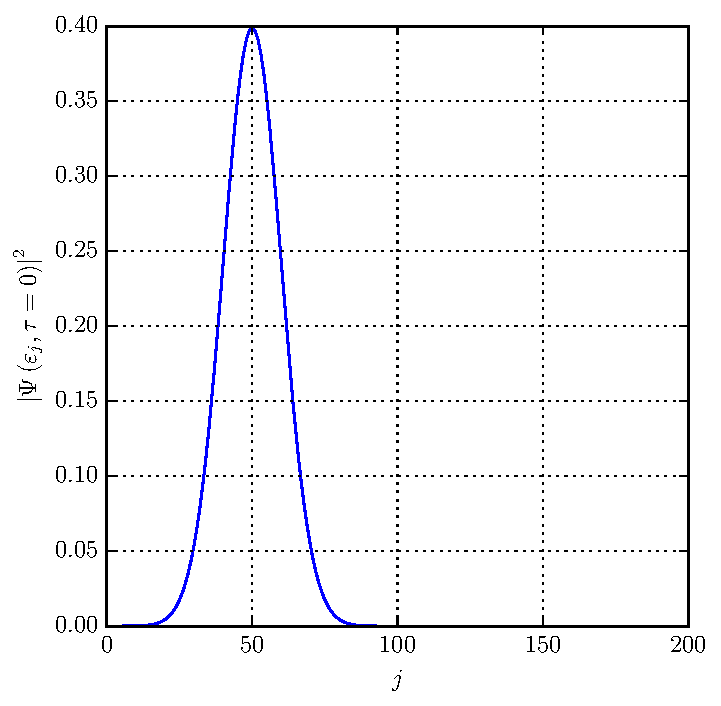
\includegraphics[width=0.5\textwidth]{Abbildungen/Anfangszustand.pdf}
\caption{Normiertes, Gauß-Wellenpacket mit $\varepsilon_0=-5$, $\sigma=1$, $k_0=5.5$ bei einer Diskretisierung von $\Delta\varepsilon=0.1$}
\label{Anfangszustand}
\end{figure}\noindent
Der Zustand zum Zeitpunkt $\tau$ wird berechnet, in dem der Anfangszustand $\frac{\tau}{\Delta \tau}$-mal mit dem Zeitwentwicklungsoperator nach Crank-Nicolson
\begin{equation}
S_H=\left(\mathbbm{1}+\frac{i}{2}H\Delta\tau\right)^{-1}
\left(\mathbbm{1}-\frac{i}{2}H\Delta\tau\right)
\end{equation}
multipliziert wird. Dabei wird außerdem in jedem Zeitschritt überprüft mit welcher Wahrscheinlichkeit sich die Welle rechts der Mitte der Potentialbarriere befindet. Daraus ergibt sich der Transmissionskoeffizient 
\begin{equation}
T=\sum_{\varepsilon_j>0} \Delta\varepsilon\left|
\Psi\left(\varepsilon_j\,,\,\tau\right)\right|^2\,.
\end{equation}
Die Betragsquadrate der Zustände zum Zeitpunkt $\tau=1$ für Potenzialbarrieren der Breite $b=1$ und der Höhe $\tilde{V}_0\in\left\lbrace 0\,,\,10\,,\,30\,,\,50\right\rbrace$
sind in Abbildung \ref{Zeitentwicklung} dargestellt.
 \begin{figure}[H]
\centering 
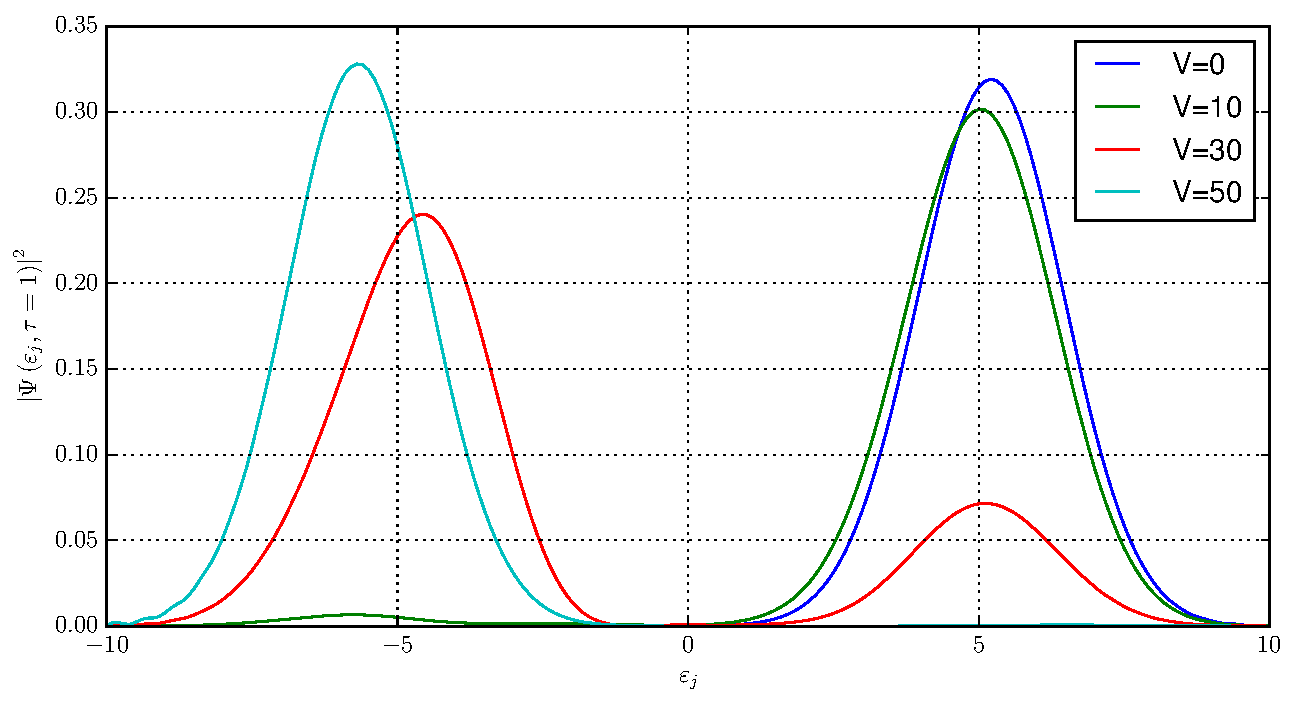
\includegraphics[width=0.9\textwidth]{Abbildungen/Zeitentwicklung.pdf}
\caption{Zeitentwicklung des normierten Gauß-Wellenpacketes mit Potentialbarrieren der Höhen $\tilde{V}_0\in\left\lbrace 0\,,\,10\,,\,30\,,\,50\right\rbrace$}
\label{Zeitentwicklung}
\end{figure}\noindent
Es ist deutlich zu erkennen, dass das Wellenpacket sich ohne Potenzialbarriere ungehindert nach rechts ausbreitet und zunehmend zerfließt, also breiter und niedriger wird. Auch für eine kleine Potenzialbarriere mit $\tilde{V_0}=10$ propagiert ein Großteil des Wellenpacketes nach rechts und nur ein sehr kleiner Anteil wird reflektiert. Für $\tilde{V_0}=30$ wird aber bereits ein Großteil des Packetes reflektiert und bei $\tilde{V_0}=50$ ist kaum noch eine Aufenthaltswahrscheinlichkeit rechts der Potenzialbarriere nachweisbar. Hier werden auch Interferenzeffekte durch die Überlagerung der einlaufenden und auslaufenden Welle sichtbar.\\ 
Der Transmissionskoeffizient ist in Abbildung \ref{Transmission} dargestellt. Hier wird deutlich, dass der Transmissonskoeffizient ohne Potenzialbarriere für große Zeiten asymptotisch gegen 1 geht. Auch für endliche Potenzialbarrieren steigt der Transmissionskoeffizient zunehmend an, wobei ein Wendepunkt vorliegt wenn der Erwartungswert in der Mitte der Potenzialbarriere , also bei $\left\langle\varepsilon_j\right\rangle=0$ angekommen ist. Ab hier nimmt die Steigung ab und der Transmissionskoeffizient nähert sich asymptotisch einem Wert kleiner als $1$.
 \begin{figure}[H]
\centering 
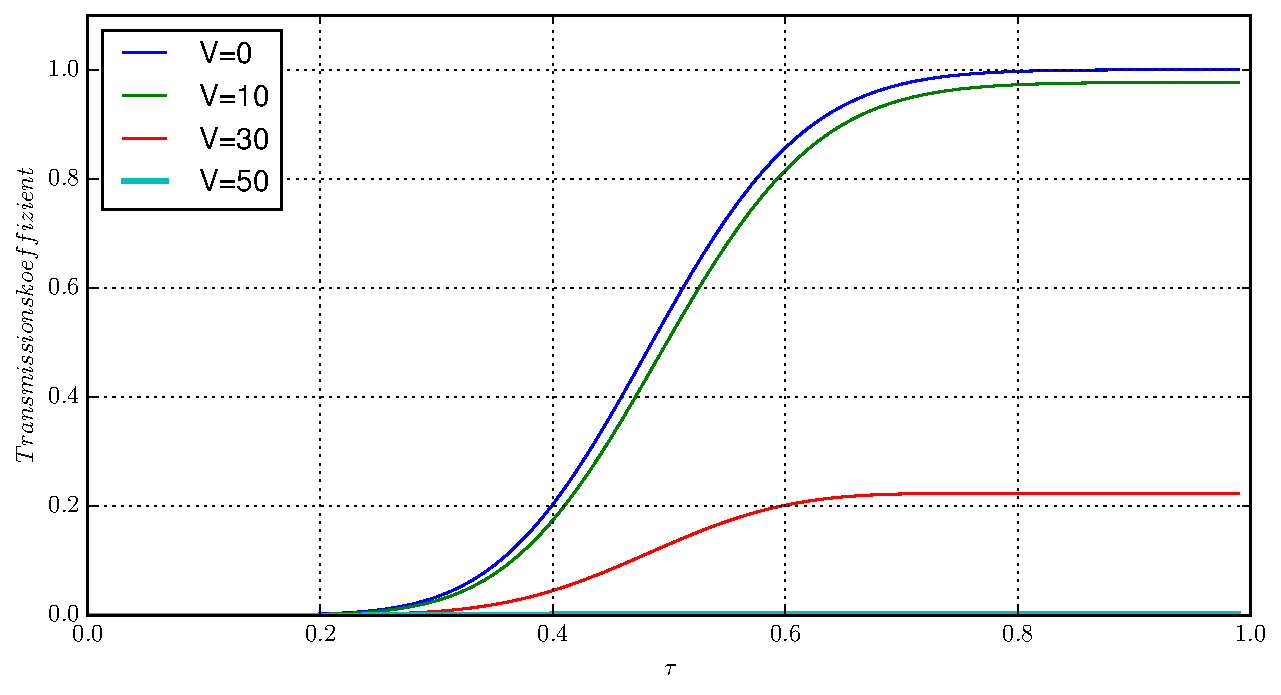
\includegraphics[width=0.8\textwidth]{Abbildungen/Transmission.pdf}
\caption{Transmissionskoeffizient des normierten Gauß-Wellenpacketes mit Potenzialbarrieren der Höhen $\tilde{V}_0\in\left\lbrace 0\,,\,10\,,\,30\,,\,50\right\rbrace$}
\label{Transmission}
\end{figure}\noindent

\section{Poisson-Gleichung}
Im Folgenden wird die zweidimensionale Poisson-Gleichung 
\begin{equation}
\left(\partial_x^2+\partial_y^2\right)\Phi\left(x,y\right)=
\rho\left(x,y\right)\label{poisson}
\end{equation}
für eine diskrete Ladungsverteilung 
\begin{equation}
\rho\left(r\right)=\sum_i q_i \delta\left(\vec{r}-\vec{r}_i\right)
\end{equation}
auf einem Quadrat $Q=\left[0\,,\,1\right]$ mittels einer Gauß-Seidel Iteration gelöst. Es wird dabei von Dirichlet-Randbedingungen, ausgegangen, also der Wert des Potentials auf den Rändern des Quadrates als konstant festgelegt. Dann kann die Poisson-Gleichung rekursiv mit der Diskretisierung $\Delta$ über 
\begin{equation}
\Phi_{j,l}^{n+1}
=
\frac{1}{4}
\left(
\Phi_{j+1,l}^{n}
+\Phi_{j-1,l}^{n+1}
+\Phi_{j,l+1}^{n}
+\Phi_{j,l-1}^{n+1}
\right)
+\frac{1}{4}\Delta\rho_{j,l}
\end{equation}
gelöst werden. Dazu wird das Quadrat in $\left(\frac{L}{\Delta}\right)^2$ Unterquadrate aufgeteilt und das Potential als $\left(\frac{L}{\Delta}\right)$-Dimensionale Matrix geschrieben. Die Ladungsdichte wird ebenfalls als $\left(\frac{L}{\Delta}\right)$-dimensionale Matrix geschrieben, wobei der jeweilige Matrixeintrag wenn in dem Punkt die $j$-te Ladung liegt durch $q_i$ gegeben ist, und sonst null beträgt. Der Rand des Potentials wird innerhalb der Iteration nicht aktualisiert, somit sind die konstanten Randbedingungen erfüllt. Außerdem wird aus dem momentanen Potential das Elektrische Feld berechnet. Da $\vec{E}\left(\vec{r}\right)=-\nabla \Phi\left(r\right)$ gilt können die $x$-Komponente und die $y$-Komponente mittels der Nachbarmatrixelemente über 
\begin{eqnarray}
\partial_x\Phi\left(x\,,\,y\right)
&=&
\frac{\Phi\left(x+\Delta\,,\,y\right)-\Phi\left(x-\Delta\,,\,y\right)}{2\Delta}
\\
\partial_y\Phi\left(x\,,\,y\right)
&=&
\frac{\Phi\left(x\,,\,y+\Delta\right)-\Phi\left(x\,,\,y-\Delta\right)}{2\Delta}
\end{eqnarray}
berechnet werden. Das Elektrische Feld auf dem Rand wird nicht berechnet, da die numerische Ableitung hier nicht definiert ist.
\\
Zunächst wird nun davon ausgegangen, dass das Potential auf dem Rand konstant null ist. Sind nun keinerlei Ladungen vorhanden, gilt also $\rho_{jl}=0$, so ist die Lösung der Poisson-Gleichung gegeben durch $\Phi\left(\vec{r}\right)=0$. Die Iteration wird in unserem Fall begonnen indem das Potential im Inneren des Quadrates auf $1$ gesetzt wird, und die Ergebnisse für Potential und $\vec{E}$-Feld nach $N=500000$ Iterationen sind als Wärmeplots in Abbildung \ref{a} dargestellt.
\begin{figure}[H]
    \centering
    \begin{subfigure}[b]{0.45\textwidth}
        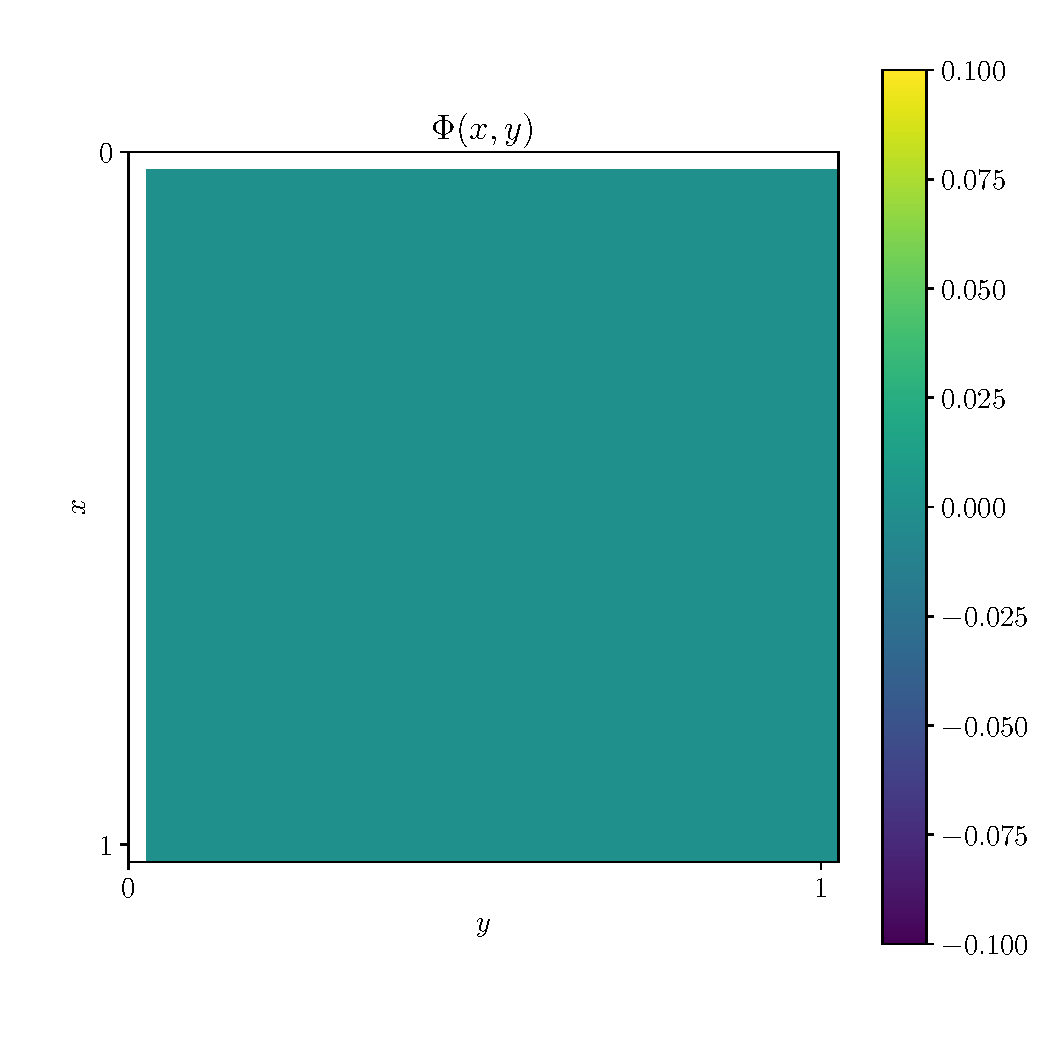
\includegraphics[width=\textwidth]{Abbildungen/Phi_a.pdf}
           \caption{$\Phi\left(\vec{r}\right)$\color{white}{$\left|\vec{E}\right|$}}
   \end{subfigure}
     \begin{subfigure}[b]{0.45\textwidth}
        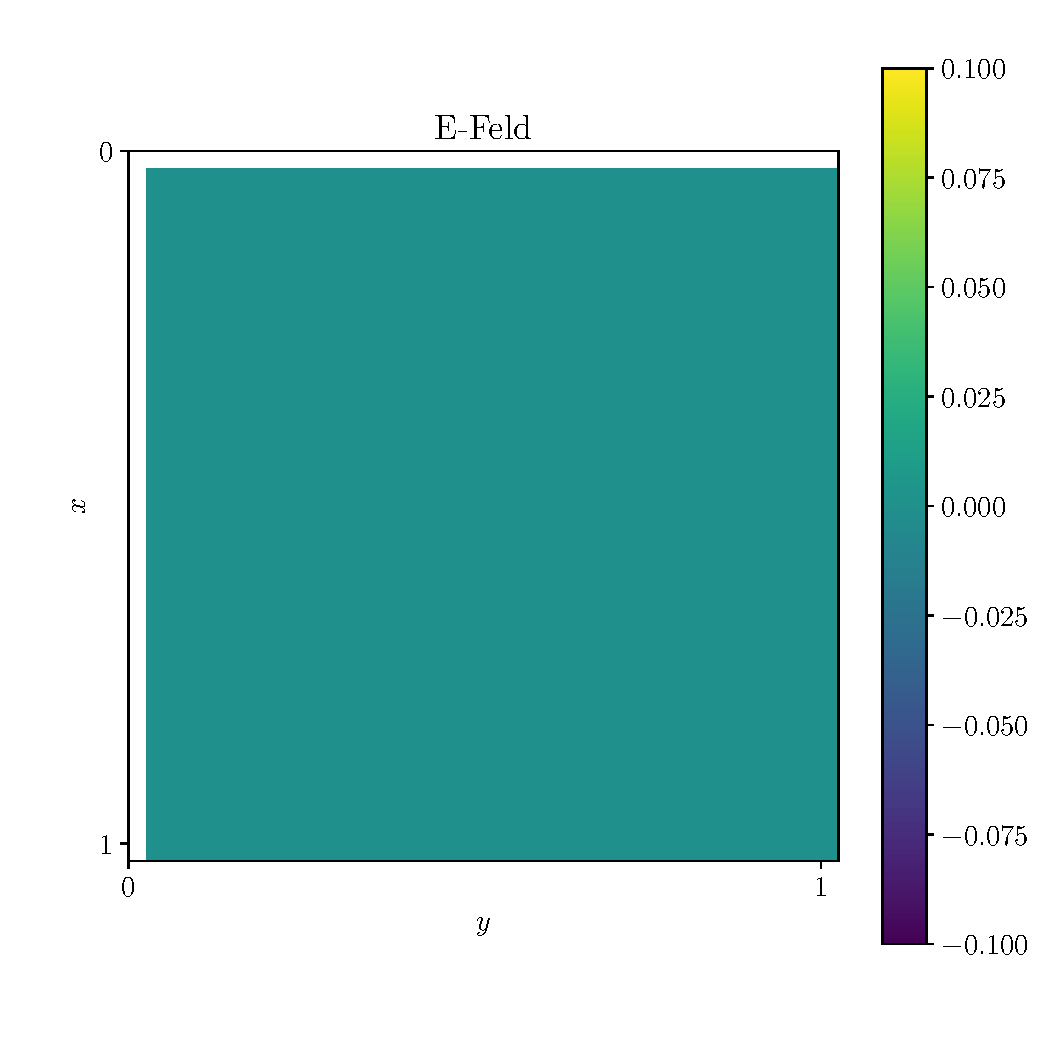
\includegraphics[width=\textwidth]{Abbildungen/E_a.pdf}
           \caption{$\left|\vec{E}\left(\vec{r}\right)\right|$}
   \end{subfigure}
   \caption{Lösung der Poisson-Gleichung für ein Potential das auf dem Rand konstant null ist und keine Ladungen vorhanden sind, bei
   $N=500000$ Iterationen  }\label{a}
   \end{figure}\noindent
Offensichtlich zeigen sowohl das Potential als auch das $\vec{E}$-Feld nach $N=500000$ Iterationen nur sehr geringe, numerische Abweichungen von Null.\\
Nun werden die Randbedingungen so verändert, dass das Potential weiterhin auf $3$ Rändern des Quadrates gleich null ist, jedoch auf dem Rand bei $\Phi\left(x,1\right)=1$ ist. Zunächst wird dieser Fall analytisch betrachtet. Dazu wird für das Potenzial der Produktansatz 
\begin{equation}
\Phi\left(x,y\right)=X\left(x\right)\cdot Y\left(y\right)
\end{equation}
gewählt, welcher eingesetzt in \eqref{poisson} auf 
\begin{eqnarray}
X''\left(x\right)\cdot Y\left(y\right)+X\left(x\right)\cdot Y''\left(y\right)&=&0
\\
\frac{X''\left(x\right)}{\cdot +X\left(x\right)}+\frac{Y''\left(y\right)}{Y\left(y\right)}
&=&0
\\
\frac{X''\left(x\right)}{X\left(x\right)}
&=&
-\frac{Y''\left(y\right)}{Y\left(y\right)}=\lambda^2
\end{eqnarray}
mit konstantem $\lambda$ führt. Damit sind die zu lösenden Differentialgleichungen gegeben durch
\begin{eqnarray}
X''\left(x\right)-\lambda^2 X\left(x\right)&=&0
\\
Y''\left(y\right)+\lambda^2 Y\left(y\right)&=&0\,.
\end{eqnarray}
Diese werden durch 
\begin{eqnarray}
 X\left(x\right)&=&A_+ e^{\lambda x} +A_- e^{-\lambda x}
 \\
  Y\left(y\right)&=&B_+ e^{i\lambda y} +B_- e^{-i\lambda y} 
\end{eqnarray}
gelöst. Die Randbedingungen führen im Produktansatz auf 
\begin{subequations}
\begin{eqnarray}
\label{1}
\Phi\left(0\,,\,y\right)=0\quad&\rightarrow&\quad X\left(0\right)=0
\\\label{2}
\Phi\left(x\,,\,0\right)=0\quad&\rightarrow&\quad Y\left(0\right)=0
\\\label{3}
\Phi\left(1\,,\,y\right)=0\quad&\rightarrow&\quad X\left(1\right)=0
\\\label{4}
\Phi\left(x\,,\,1\right)=1\quad&\rightarrow&\quad X\left(x\right)
\cdot Y\left(1\right)=1\,.
\end{eqnarray}
\end{subequations}
Aus \ref{1} und \ref{2} folgt $A_+=-A_-=A$ und $B_+=-B_-=B$ und somit 
\begin{eqnarray}
 X\left(x\right)&=&A\left( e^{\lambda x} - e^{-\lambda x}\right)
 \\
  Y\left(x\right)&=&B\left( e^{i\lambda y} - e^{-i\lambda y} \right)\,.
\end{eqnarray}
Aus \ref{3} folgt außerdem
\begin{equation}
X\left(1\right)=A\left(e^{\lambda}-e^{-\lambda}\right)=0\quad\rightarrow
\quad
\lambda=n\pi i
\Mit 
n \in \mathbb{N}\,,
\end{equation}
was auf 
\begin{eqnarray}
 X\left(x\right)&=&A_n\left( e^{i n\pi  x} - e^{-i n\pi x}\right)
 =2A_n i\sin\left(n\pi x\right)
 \\
  Y\left(x\right)&=&B_n\left( e^{- n\pi y} - e^{n\pi y} \right)
  =-2B_n\sinh\left(n\pi y\right)
\end{eqnarray}
führt. Nun muss lediglich noch Die Anfangsbedingung \eqref{4} erfüllt werden. Dazu betrachten wir nun aber wieder die Funktion $\Phi\left(x\,,\,y\right)$, welche sich als Überlagerung aller Produktlösungen ergibt:
\begin{equation}
\Phi\left(x\,,\,y\right)
=
\sum_n 
\left(-4 A_n B_n i\right)
\sinh\left(n\pi y\right)
\sin\left(n\pi x\right)
=
\sum_n 
c_n
\sinh\left(n\pi y\right)
\sin\left(n\pi x\right)\label{allg}
\end{equation} 
Nach \eqref{4} wird nun gefordert, dass
\begin{equation}
\Phi\left(x\,,\,1\right)
=
\sum_n 
{\color{dunkelgr}{
c_n
\sinh\left(n\pi \right)}}
\sin\left(n\pi x\right)\overset{!}{=}1\label{rb}
\end{equation} 
Der grüne Teil der Gleichung ist lediglich abhängig vom Summationsindex $n$, Gleichung \eqref{rb} kann daher mit der Definition einer beliebigen $L$-periodischen Fourier-Reihe in Sinus-Cosinus-Form, welche durch
\begin{equation}
f(x)=\frac{a_0}{2}+\sum_{k=1}^\infty a_k\cos\left(kx\right)+b_k\sin\left(kx\right)\label{Fourier}
\end{equation}
gegeben ist, verglichen werden. Gleichung \eqref{rb} entspricht \eqref{Fourier} mit 
\begin{equation}
b_k=c_n\sinh\left(n\pi\right)\Und
k=n\pi
\Und
a_k=0\,\,\forall\,\,k\,.\label{umform}
\end{equation}
Der Fourierkoeffizient $b_k$ für eine $L$-Periodische Funktion $f(x)$ ist gegeben durch 
\begin{equation}
b_k=\frac{2}{L}\int_0^L f(x)\sin\left(kx\right)\,\mathrm{d}x
\fur
m\geq 1
\end{equation}
und mit $f(x)=1$ und $L=1$ ergibt sich
\begin{equation}
b_k=2\int_0^1 \sin\left(kx\right)\,\mathrm{d}x
=2\left[\frac{-\cos\left(kx\right)}{k}\right]_{x=0}^{x=1}
=\frac{2}{k}\left(1-\cos\left(k\right)\right)\,.
\end{equation}
Nun können die Umformungen aus \eqref{umform} rückgängig gemacht werden, sodass für den Koeffizienten $c_n$ der Zusammenhang
\begin{eqnarray}
b_k=\frac{2}{k}\\\frac{2}{k}\left(1-\cos\left(k\right)\right)&=&c_n\sinh\left(n\pi\right)\\
\frac{2}{n\pi}\left(1-\cos\left(n\pi\right)\right)&=&c_n\sinh\left(n\pi\right)\\
\frac{2\left(1-\cos\left(n\pi\right)\right)}{n\pi\sinh\left(n\pi\right)}
&=&c_n
\end{eqnarray}
gefunden wird. Dies wiederum kann in Gleichung \eqref{allg} eingesetzt werden, und das Potential ergibt sich zu 
\begin{equation}
\Phi\left(x\,,\,y\right)
=
\sum_n 
\frac{2\left(1-\cos\left(n\pi\right)\right)}{n\pi\sinh\left(n\pi\right)}
\sinh\left(n\pi y\right)
\sin\left(n\pi x\right)\label{poten}
\end{equation}
Dieses Potential ist als Wärmeplot in Abbildung \ref{ana} dargestellt, wobei für jedes Matrixelement nur die ersten $200$ nicht verschwindenden Terme der Reihe \eqref{poten} berechnet wurden. In Abbildung \ref{b} ist die numerische Lösung mittels Gauß-Seidel-Iteration dargestellt.
 \begin{figure}[H]
\centering 
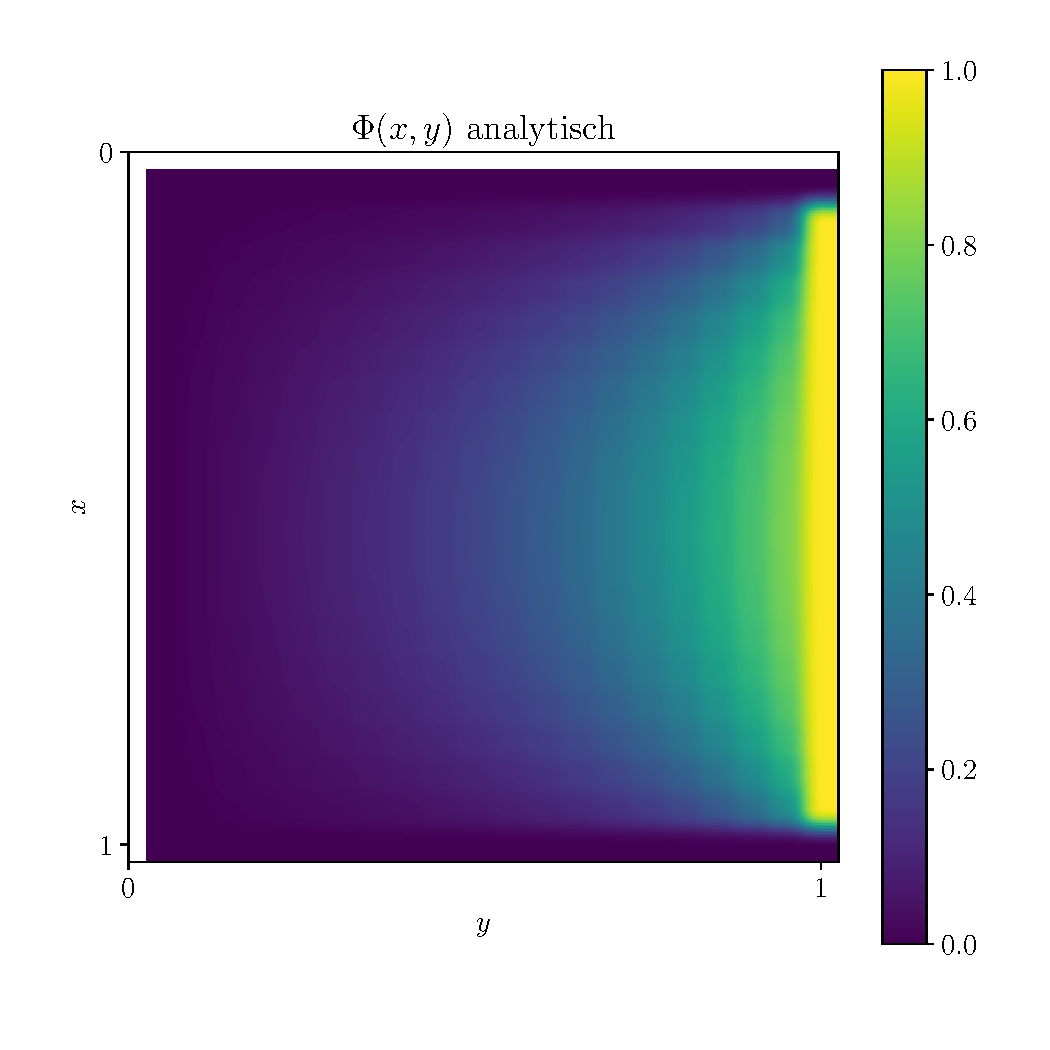
\includegraphics[width=0.45\textwidth]{Abbildungen/Phi_b_ana.pdf}
\caption{Analytische Lösung der Poissongleichung für $\Phi\left(0\,,\,y\right)=0\,,\,
\Phi\left(x\,,\,0\right)=0\,,\,
\Phi\left(1\,,\,y\right)=0\,,\,
\Phi\left(x\,,\,1\right)=1$ mit $200$ nicht verschwindenden Termen.}
\label{ana}
\end{figure}\noindent
\begin{figure}[H]
    \centering
    \begin{subfigure}[b]{0.45\textwidth}
        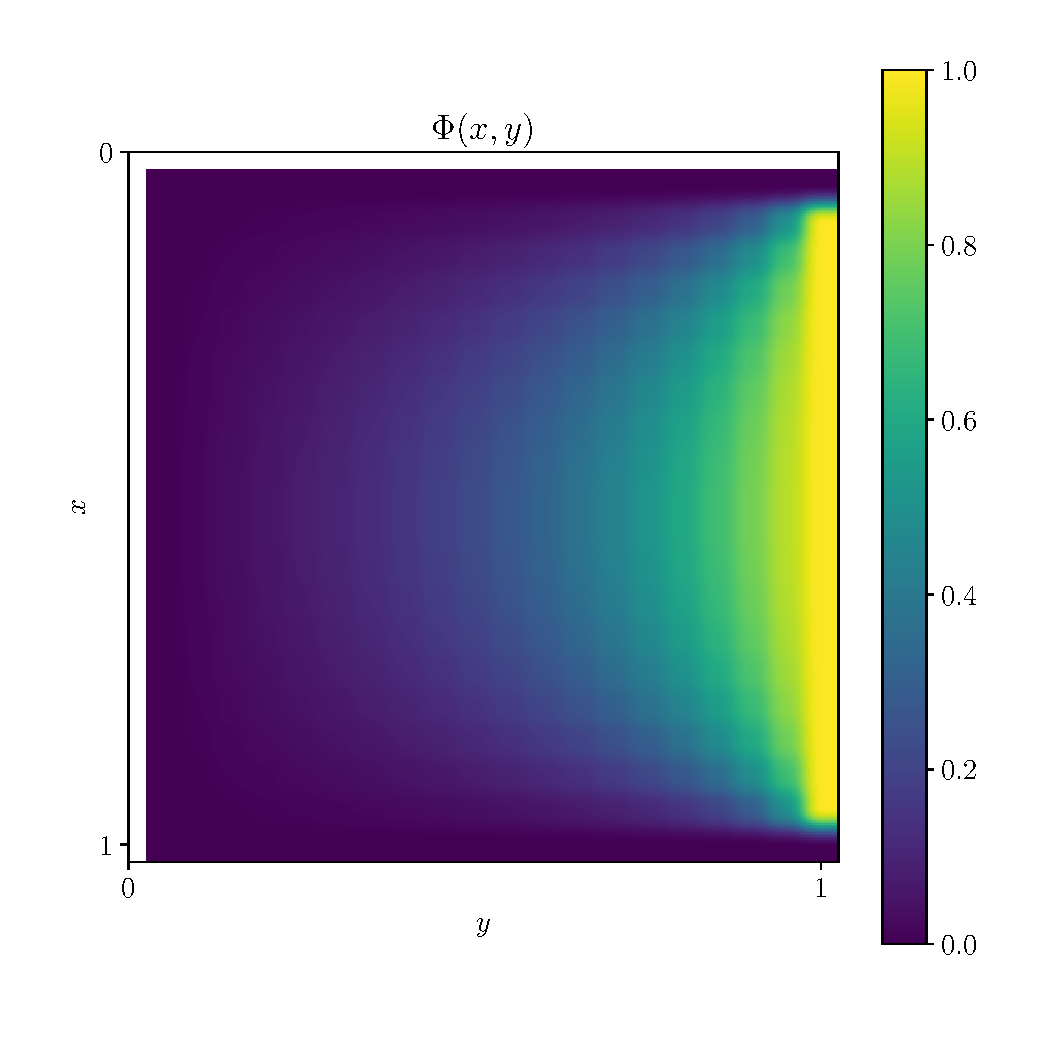
\includegraphics[width=\textwidth]{Abbildungen/Phi_b.pdf}
           \caption{$\Phi\left(\vec{r}\right)$\color{white}{$\left|\vec{E}\right|$}}
   \end{subfigure}
     \begin{subfigure}[b]{0.45\textwidth}
        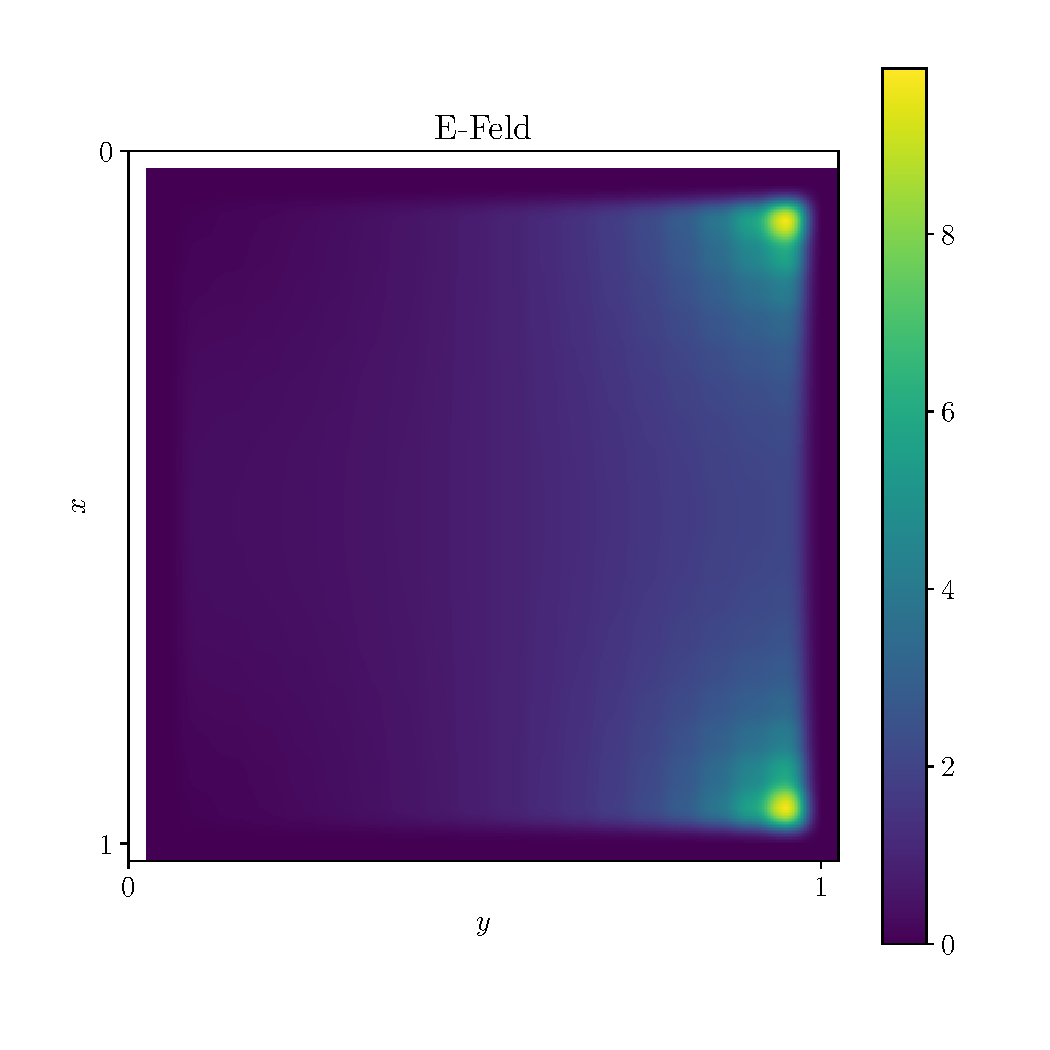
\includegraphics[width=\textwidth]{Abbildungen/E_b.pdf}
           \caption{$\left|\vec{E}\left(\vec{r}\right)\right|$}
   \end{subfigure}
   \caption{Numerische Lösung der Poisson-Gleichung für ein Potential mit $\Phi\left(0\,,\,y\right)=0\,,\,
\Phi\left(x\,,\,0\right)=0\,,\,
\Phi\left(1\,,\,y\right)=0\,,\,
\Phi\left(x\,,\,1\right)=1$ bei
   $N=500000$ Iterationen  }\label{b}
   \end{figure}\noindent
Obwohl die Wärmeplots des Potentials in der analytischen und der numerischen Lösung große Ähnlichkeit aufweisen, zeigt die Berechnung von $\Phi_{jl}^{numerisch}-\Phi_{jl}^{analytisch}$ Abweichungen in der Größenordung von $10^{-2}$. Ob dies auf den numerischen Fehler der Iteration oder den Abbruch der Summe in der analytischen Rechnung zurück zu führen ist, ist uns jedoch nicht klar. \\
Zuletzt wurde die Poissongleichung noch für ein Potential betrachtet, dass wie in Aufgabenteil a) auf allen Rändern konstant null ist. Nun ist die Ladungsdichte jedoch nicht null sondern es liegt eine diskrete Ladung mit $q=+1$ in der Mitte des Quadrates vor. Die Wärmeplots des numerisch gefundenen Potentials und des Elektrischen Feldes sind in Abbildung \ref{c} dargestellt.
\begin{figure}[H]
    \centering
    \begin{subfigure}[b]{0.45\textwidth}
        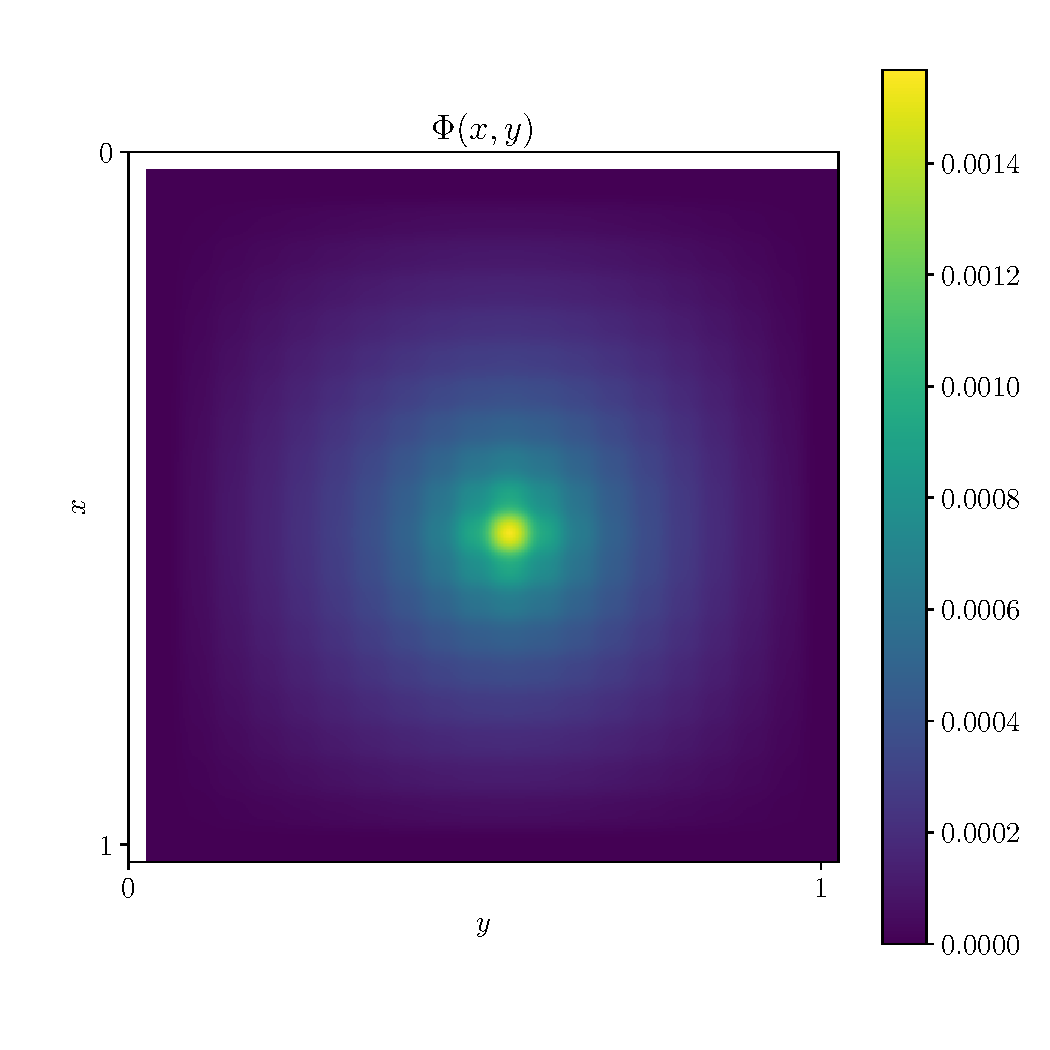
\includegraphics[width=\textwidth]{Abbildungen/Phi_c.pdf}
           \caption{$\Phi\left(\vec{r}\right)$\color{white}{$\left|\vec{E}\right|$}}
   \end{subfigure}
     \begin{subfigure}[b]{0.45\textwidth}
        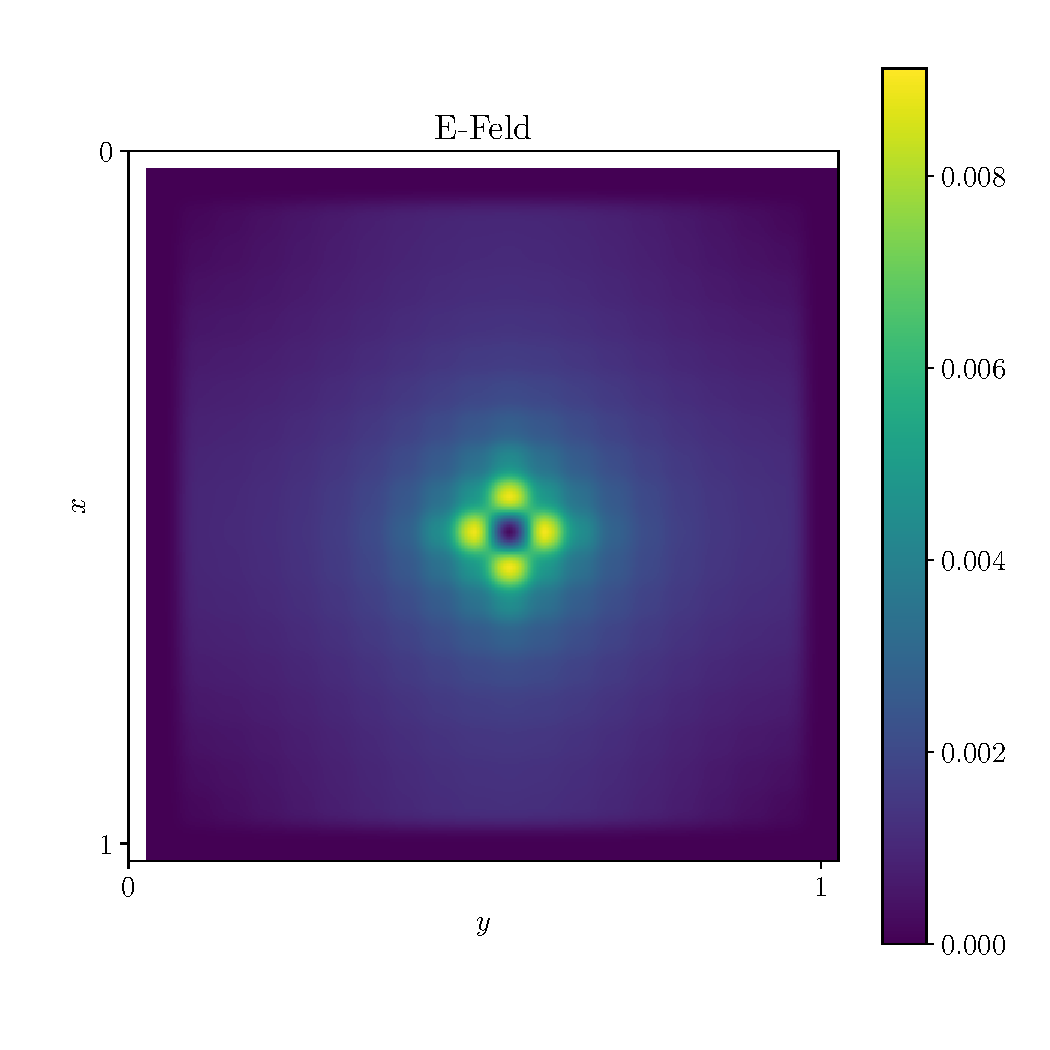
\includegraphics[width=\textwidth]{Abbildungen/E_c.pdf}
           \caption{$\left|\vec{E}\left(\vec{r}\right)\right|$}
   \end{subfigure}
   \caption{Numerische Lösung der Poisson-Gleichung für ein Potential mit $\Phi\left(0\,,\,y\right)=
\Phi\left(x\,,\,0\right)=0
\Phi\left(1\,,\,y\right)=0
\Phi\left(x\,,\,1\right)=0$ und einer Ladung bei $\left(x=0.5\,,\,y=0.5\right)$ bei
   $N=500000$ Iterationen. }\label{c}
   \end{figure}\noindent 


% >>> Anhang <<<

\begin{appendix}
%\input{Kapitel/Anhang}
\end{appendix}




\end{document}